\documentclass{SelimArticle}
%!TEX root = main.tex

%%%%%%%%%%%%%%%%%%%%%%%%%%%%%%%
% Additional Packages/Options %
%%%%%%%%%%%%%%%%%%%%%%%%%%%%%%%
% \setlist{nosep}
\hypersetup{hidelinks}

%%%%%%%%%%%%%%%%%
% Title Options %
%%%%%%%%%%%%%%%%%
\usepackage{mypage}
\school{McGill University}
\course{Computational Aerodynamics}
\coursenum{MECH 539}
%Add \\[0.3cm] for new line.
\title{Project 5}
\student{Selim \textsc{Belhaouane}}
\studentnum{260450544}
\date{\today}

%%%%%%%%%%%%%%%%%%%%%%%%%
% Additional Formatting %
%%%%%%%%%%%%%%%%%%%%%%%%%
%Horizontal line below section.
\sectionfont{\sectionrule{0pt}{0pt}{-5pt}{0.8pt}}
%Section numbering depth. Value of 2 means numbering ends with subsections.
\setcounter{secnumdepth}{3}
%Table of contents section depth. Same as above.
\setcounter{tocdepth}{2}
\numberwithin{equation}{section}
\numberwithin{figure}{section}

\newcommand{\ra}[1]{\renewcommand{\arraystretch}{#1}}
\begin{document}
\mytitlepage
\newpage
% Begin writing here.
\newcommand{\pexit}{\ensuremath{p_{\mathrm{exit}}}}
\section*{Solver Information}
\begin{description}[noitemsep]
    \item[Programming Language:] Fortran
    \item[Precision:] Double
    \item[Convergence Criteria:] $r^{(k+1)} < 10^{-14}$
\end{description}

The residual for each iteration is calculated as:
$$
r^{(k+1)} = \max_i \left( \rho^{(k+1)}_i - \rho^{(k)}_i \right)
$$

\newpage
\section{Number of panels}

The panel method essentially consists in discretizing an integral with a finite linear combination of
simple solutions, in this case doublets with a constant strength over the length of each panel.
Thus, it is expected that increasing the number of terms in the sum would increase the
accuracy of the discrete solution relative to the analytical one. Moreover, panels all have
equal lengths in PABLO -- this is important.

The pressure distributions are shown in~\Cref{fig:q1}. Most of the discrepancy in pressure
results is found at the airfoil's extremities, specifically the leading edge and trailing edge.
This can be explained by two factors:
\begin{enumerate}
    \item The increased curvature of the airfoil geometry at the leading edge, which requires a higher
        number of panels to be modelled correctly by flat panels.
    \item The increased curvature of the pressure distribution at the leading and trailing edge, which
        again requires a higher number of panels since panels are of constant strength.
\end{enumerate}
Unfortunately, determining the minimum necessary number of panels to acquire a reasonably accurate
solution would require eyeballing.

Lift and drag coefficients are tabulated in~\Cref{tab:q1}. It should be noted that the
precision on the drag coefficients output by PABLO was limited to 4 digits. Thus, lift coefficient
data is more relevant. From these results, one may say that using as little as 50 panels is sufficient
if the user is fine with a $\Delta C_L$ of 1\%. $\Delta C_L$ as a function of the number of panels
NP is calculated as follows:
\begin{equation*}
    \Delta C_L(NP) = \frac{|C_L(NP) - C_L(100)|}{C_L(100)}
\end{equation*}
Of course, this is dependent on the geometry and flow parameters.
\begin{table}
    \centering
    \caption{Effect of number of panels (NP) on lift and drag coefficients. $\Delta C_L$ and $\Delta C_D$
        are calculated with respect to the values obtained for NP = 100.}
    \label{tab:q1}
    \input{tableq1}
\end{table}

\begin{figure}[H]
    \centering
    \includegraphics[width=1.0\textwidth]{./figs/q1.pdf}
    \caption{Effect of number of panels (NP) on pressure distribution over the airfoil and at
        select locations.}\label{fig:q1}
\end{figure}


\newpage
\section{Comparison with experimental data}
Numerical data from the provided reference could only be obtained for angles of
attack of 0 and 10 degrees, thus the comparison will be performed for these
angles instead. Moreover, said data is only available for the upper surface.

\Cref{fig:q2} compares the inviscid and viscous results, using PABLO, against
the experimental data.

\begin{figure}
    \centering
    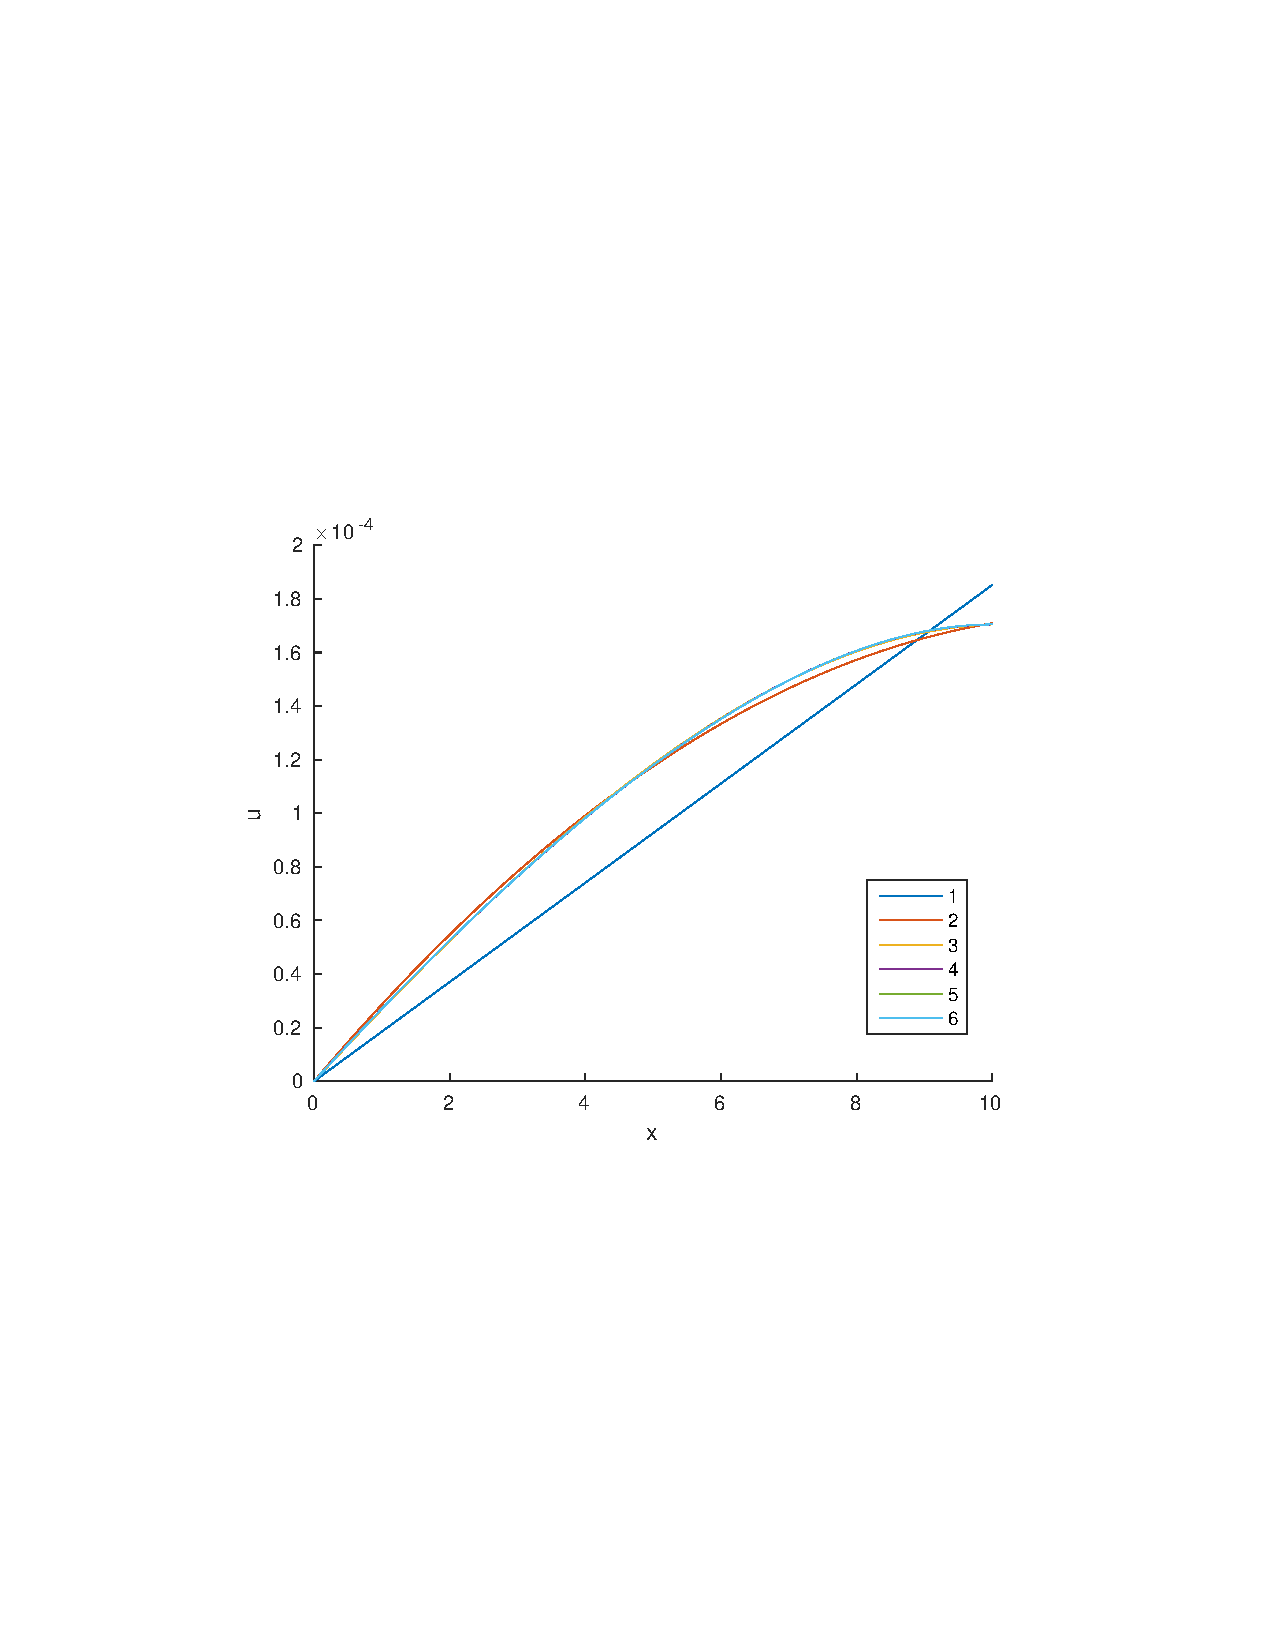
\includegraphics[width=1.0\textwidth]{./figs/q2}
    \caption{Comparison of NASA's experimental data with PABLO's viscous
        and inviscid results. The latter two results are identical.}\label{fig:q2}
\end{figure}

\subsection{Effect of viscosity}
The first thing to notice is that PABLO's viscous and inviscid solutions are exactly
the same. As a matter of fact, toggling the ``Viscous'' has absolutely no effect on
the computed pressure distribution. The boundary layer (BL) solver and potential flow (PF)
solver are completely decoupled and the overall solve is not iterative, meaning both
solvers are only run once. Specifically, the velocity field is output from the PF solver
and input into the BL solver.

\subsection{Comparison}


\newpage
\section{Aerodynamic performance}
Aerodynamic coefficients are tabulated in~\Cref{tab:aero}. Results were compared
to a 1988 paper by Ladson~\cite{ladson1988effects}. This paper presents experimental data of
the low-speed aerodynamic characteristics of the NACA 0012 airfoil, which is
in line with this project.

The rest of this section will be split between an analysis of the MECH 539 results alone and
a comparison between MECH 539 and experimental data.


\subsection{MECH 539 results}
Let's look at lift first. Most textbooks will explain lift as a difference in pressure
between the upper and bottom surface, which results in a net upwards force. In other words,
there is usually no mention of viscous forces when considering lift. Thus, it makes sense
that, according to~\Cref{tab:aero}, $c_{l_p}$ is essentially the sole contributor to
lift.

Now, the same cannot be said of drag, where $c_{d_f}$ and $c_{d_p}$ contribute almost
equally to the total drag. Additionally, it can be said that viscous forces
primarily contribute to drag, while pressure forces have a large relative impact on both
lift and drag.

Finally, it can be seen that $c_l$ is around 2 orders of magnitude higher than $c_d$, i.e.
$l/d \approx 100$.
\subsection{Comparison with experimental}
Experimental data in~\Cref{tab:aero} was obtained from Table I
in~\cite{ladson1988effects}. The latter table lists values of lift and drag coefficients
-- but not the contributions from viscous and pressure forces -- at a Reynolds number of 2
million and Mach number of 0.15 for various angles of attack. While the Mach number
does not correspond to that of the provided MECH 539 results (0.1) both are low enough
that the flow is essentially incompressible, making the Reynolds number a more important
value to match -- and these match exactly. In other words, changes in Mach number
at subsonic speeds should not be expected to significantly affect aerdoynamic performance
as long as the Reynolds number is kept constant.  Finally, the experimental
data needed to be interpolated in order to obtain values at $\alpha = 8.0$.

The MECH 539 and Ladson results are of the same orders of magnitude but differ by around
3\% and 20\% for lift and drag respectively. Of course, sources of discrepancy in
the experimental data are always expected, especially in the presence of turbulent flow
since it is inherently unsteady and very sensitive to inputs~\cite{pope}.

Moreover, as will be discussed in~\Cref{sec:bl}, the numerical simulation predicts
three zones of recirculation on the airfoil. Since a RANS solver was used, it is expected
that values should be slightly off, as was discussed in class.
\begin{table}
    \centering
    \caption{Aerodynamic coefficients of provided data and experimental data from
        ~\cite{ladson1988effects}.}
    \label{tab:aero}
    
\begin{tabular}{@{} l ccc c ccc}
\toprule
 & \multicolumn{3}{c}{Lift} & \phantom{a} & \multicolumn{3}{c}{Drag}\\
\cmidrule{2-4}\cmidrule{6-8}
Source & Pressure & Viscous & Total && Pressure & Viscous & Total\\
\midrule
MECH 539 & 0.8091 & -0.0001 & 0.8089 && 0.0048 & 0.0049 & 0.0098\\
Ladson & - & - & 0.8386 && - & - & 0.0079\\
\bottomrule
\end{tabular}

\end{table}

\newpage
\section{Airfoil comparison}
\subsection{Drag polar}
The drag polars are shown in~\Cref{fig:q4_polars}. Typically, a higher lift-to-drag (L/D) ratio
is one of the most imperative goals in airfoil design.
Since constant L/D lines have also been plotted, the comparison becomes straight-forward:
\begin{itemize}
    \item The NACA 0012 airfoil has a lower L/D ratio than the other two airfoils
        for any value of lift coefficient.
    \item Except at low lift coefficients, the DAE31 airfoil is the best airfoil in terms
        of L/D ratio.
\end{itemize}
The other factor that may be considered is the following: it is desirable for an airfoil
to attain high lift at relatively low angles of attack. This is especially true when
doing simulations with a potential flow solver, since it cannot predict stall although
we know it occurs for all airfoils at some point. Comparing airfoils this way basically
leads to the same ranking as above.
\begin{figure}
    \centering
    \includegraphics[width=\textwidth]{./figs/q4_polars}
    \caption{Drag polars for all three airfoils. Drag at $C_L = 1$ is shown as
        empty circle.}\label{fig:q4_polars}
\end{figure}

\subsection{Drag at fixed lift}
The drag at lift coefficient equal to 1.0 for all three airfoils is tabulated in
~\Cref{tab:q4}. It has been interpolated using the data shown in the drag polars
plot. The table shows that the DAE31 airfoil exhibits the lowest drag coefficient
at that particular lift coefficient. GA(W) is the second best and NACA0012 is the
worst out of the three.

For the sake of completeness, it should be noted that low drag coefficients are usually
desirable when designing airfoils for aerodynamics.
\begin{table}
    \centering
    \caption{Drag coefficients at equivalent lift coefficient of 1.0}
    \label{tab:q4}
    \input{tableq4}
\end{table}

\subsection{Pressure distribution}
The pressure distribution for all airfoils is shown on~\Cref{fig:q4_cp}. The following
observations can be made:
\begin{itemize}
    \item The NACA0012 and GA airfoils produce most of their lift close to the leading edge;
        that is where the difference in pressure between top and bottom surface is greatest.
        In fact, compared to DAE31, GA and NACA exhibit large peaks in pressure
        right at the leading edge, after which the pressure quickly increases on the top surface
        and decreases on the bottom surface.
    \item GA produces more lift near the trailing edge than NACA, which produces
        low lift after around 80\% of the length.
    \item The DAE31 airfoil produces most of its lift over the first 60\%. The pressure
        on the bottom surface remains relatively constant over most of the length, and the
        pressure on the top surface decreases way more gradually than for the other two
        airfoils.
\end{itemize}

\begin{figure}
    \centering
    \includegraphics[width=\textwidth]{./figs/q4_cp}
    \caption{Pressure distribution for all three airfoils at angle of attack of
        4 degrees.}\label{fig:q4_cp}
\end{figure}

\subsection{Skin friction}
Skin friction plots are shown in~\Cref{fig:q4_cf}. Transition locations are also shown.
It can be seen that, on the upper surface, the flow transitions at around 15\%
for both NACA and GA while the transition occurs at 37\% for DAE. The effect
of transition on skin friction coefficient is easy to see: transition leads to a sharp increase
in skin friction coefficient. In fact, that is how it was detected. This can physically
be explained by the fact that turbulent flow has a larger velocity gradient in the normal
direction, mathematically written as $\partial u/\partial y$ in this case, than laminar flow.
The shear stress at the wall $\tau_w$ is given by:
$$
    \tau_w = \mu \left(\frac{\partial u}{\partial y}\right)_{y=0}
$$
and thus increases linearly with $\partial u/\partial y$. The skin friction coefficient
is nothing but a non-dimensionalized $\tau_w$.

The transition location can also be linked to the pressure distribution plots in the previous
section as follows:
transition leads to a sharp increase in pressure. In other words, the earlier the transition
the earlier the pressure tends to increase back up to freestream conditions. Of course, this
matches the results shown in~\Cref{fig:q4_cp}, meaning that $C_P$ for DAE stays relatively
high much longer than for GA and NACA.

The same can be said for the lower surface, except that in case pressure decreases back to
freestream value when transition occurs. Interestingly, there is no transition on the lower surface
for DAE! Consequently, the lower surface pressure stays relatively constant over most of the
airfoil's length.

Finally, the following conclusion can be made: delaying the transition as much
as possible leads to better overall aerodynamic performance.
\begin{figure}[H]
    \centering
    \includegraphics[width=\textwidth]{./figs/q4_cf}
    \caption{Skin friction coefficient for all airfoils at an angle of attack of
        4 degrees.}\label{fig:q4_cf}
\end{figure}


\newpage
\section{Further investigation of boundary layer}
The dimensionless velocity profile is shown in~\Cref{fig:uplus_mid}.
As discussed in~\Cref{sec:bl}, the flow can be said to be somehwat turbulent.

\begin{figure}
    \centering
    \includegraphics[width=0.85\textwidth]{./figs/uplus_mid.pdf}
    \caption{Dimensionless velocity profile at the middle of the airfoil.}
    \label{fig:uplus_mid}
\end{figure}

\end{document}
